\scanpage{139}
\mspage{22}
LEMMA 9. Let $(R^*,M^*)$ be an immediate quadratic trans-
form of $R$ and let $\deleted{x_1}\inserted{z_1},\ldots,\deleted{x_n}\inserted{z_n}$ be a minimal basis of
$R$. Then there exists $i$ such that $z_j/z_i\in R^*$ for
$j=1,\ldots,n$; and if we choose any one such value of
$i$ then setting $S=R[z_1/z_i,\ldots,z_n/z_i]$ we have that
$R^*\supset S$, $N=S\cap M^*$ is a maximal ideal in $S$ containing
$z_i$, $R^*=S_N$, $M^*=NR^*$, $MR^*=z_iR^*$ and $z_i$ is part of
a minimal basis of $M^*$. Also $R^*\ne R$.
\margin{small ``zed''}

\uline{Proof}. By definition there exists $x\in M$, $x\notin M^2$ such that
$R^*$ is the quotient ring of $R[Mx^{-1}]$ with respect to a maximal
ideal containing $x$. Let $v$ be a valuation of $K$ having center
$M^*$ in $R^*$. Then $z_j/x\in R^*$ implies that $v(z_j/x)\ge0$ for all
$j$ and hence $v(x)=v(M)$. Since $z_1,\ldots,z_n$ is a basis of $M$,
there exists $i$ such that $v(z_i)=v(M)=v(x)$ and then
$v(z_i/x)=0$ and this in view of the fact that $z_i/x$ is in $R^*$
implies that $z_i/x$ is a unit in $R^*$ and hence $x/z_i$ is in $R^*$
which in turn implies that $z_j/z_i=(z_j/x)(x/z_i)$ is in $R^*$ for
all $j$. Now fix $i$ such that $z_j/z_i$ is in $R^*$ for all $j$ and
let $S=R[z_1/z_i,\ldots,z_n/z_i]$. Then $R^*\supset S$. Let $N=S\cap M^*$.
\deleted{The}\inserted{Then} canonically $R^*/M^*\supset S/N\supset R/M$; and since by Lemma 1, $R^*/M^*$
is algebraic over $R/M$, $S/N$ must be algebraic over $R/M$. Since
$z_i\in M^*\cap S=N$, by Lemma 1 we conclude that $N$ is a maximal
ideal in $S$. Let $R_{\deleted{\unsure{*}}\inserted{1}}=S_N$ and $M_1=NS$. Then $R^*$ has center
\margin{$1$}
\figure{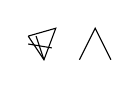
\begin{tikzpicture}\draw (0,0)--(.2,-.3)--(.35,.1)--(0,0);\draw (0,-.1)--(.3,-.15);\draw (.1,0)--(.2,-.3);\draw (.65,-.3)--(.85,.1)--(1.05,-.3);\end{tikzpicture}}
$M_1$ in $R_1$. Now $v$ also has center $M_1$ in $R_1$ and $x/z_i$ is
in $R_1$ and $v(x/z_i)=0$ which tells us that $x/z_i$ is a unit in
$R_1$. Hence $R[Mx^{-1}]\subset R_1$ and $M^*\cap R[Mx^{-1}]=(M_{\unsure{V|v}}\cap R^*)\cap R[Mx^{-1}]=$
$M_{\unsure{V|v}}\cap R[Mx^{-1}]=(M_{\unsure{V|v}}\cap R_1)\cap R[Mx^{-1}]=M_1\cap R[Mx^{-1}]$. Therefore
\mspage{138}
